\documentclass[aspectratio=169, t]{beamer}

\usepackage[utf8]{inputenc}
\usepackage[T1]{fontenc}
\usepackage[french]{babel}
\usepackage{booktabs}
\usepackage{graphicx}
\usepackage{tikz}
\usetikzlibrary{positioning, arrows.meta, fit, calc, shapes.geometric}
\usepackage{hyperref}
\usepackage{colortbl}
\usepackage{array}
\usepackage{xcolor}

\usetheme[language=french, progressbar, sectiontoc]{uae}
\beamertemplatenavigationsymbolsempty
\setbeamercovered{transparent}

\definecolor{GreenA}{HTML}{2D6A4F}
\definecolor{GreenPale}{HTML}{D8F3DC}
\definecolor{OrangeWarn}{HTML}{E07B54}
\definecolor{OrangePale}{HTML}{FDEED9}
\definecolor{BlueLight}{HTML}{EBF4FA}
\definecolor{RowHL}{HTML}{FFF9C4}

\newcommand{\badge}[2]{%
  \tikz[baseline=(x.base)]\node[fill=#1,rounded corners=3pt,
    inner xsep=4pt,inner ysep=2pt,font=\scriptsize\bfseries,
    text=white](x){#2};%
}
\newcommand{\badgegreen}[1]{\badge{GreenA}{#1}}
\newcommand{\badgeorange}[1]{\badge{OrangeWarn}{#1}}
\newcommand{\badgeblue}[1]{\badge{UAEDarkBlue}{#1}}
\newcommand{\badgegold}[1]{\badge{UAEAccentGold}{#1}}

\renewcommand{\titleframe}{%
  \begin{frame}[plain,noframenumbering]
    \begin{tikzpicture}[remember picture,overlay]
      \fill[UAEDarkBlue] (current page.north west)
        rectangle ([yshift=-2.6cm]current page.north east);
      \fill[UAELightBlue] ([yshift=-2.6cm]current page.north west)
        rectangle ([yshift=-2.72cm]current page.north east);
      \fill[UAEAccentGold] ([yshift=-2.72cm]current page.north west)
        rectangle ([yshift=-2.82cm]current page.north east);
      \node[anchor=west] at
        ([xshift=0.7cm,yshift=-1.35cm]current page.north west){%
          
\includegraphics[height=1.55cm]{logo_uae_ensa.png}};
      \node[anchor=center,text=white,align=center] at
        ([yshift=-1.35cm]current page.north){%
          \normalsize\textbf{Université Abdelmalek Essaâdi}\\[0.15cm]
          {\small École Nationale des Sciences Appliquées — Tétouan}};
      \node[anchor=east] at
        ([xshift=-0.7cm,yshift=-1.35cm]current page.north east){%
          \IfFileExists{logo-webvoice.png}{%
            
\includegraphics[height=1.35cm]{logo-webvoice.png}%
          }{%
            \tikz\node[draw=none]{};
          }%
        };
    \end{tikzpicture}
    \vspace{2.4cm}
    \begin{center}
      {\LARGE\bfseries\color{UAEDarkBlue}\inserttitle}\\[0.25cm]
      {\large\bfseries\color{UAELightBlue}\insertsubtitle}\\[0.45cm]
      \begin{minipage}{0.92\textwidth}
        \small
        \begin{tabular}{@{}ll@{}}
          \textbf{Réalisé par :} EL ASSAL Douae & \textbf{Entreprise d'accueil :} WEBVOICE (Tanger) \\
          \textbf{Filière :} Génie Informatique (2\textsuperscript{e} année) & \textbf{Encadrant entreprise :} M. Hatim BENHADDOU \\
          \textbf{Année :} 2025–2026 & \textbf{Tuteur pédagogique :} Prof. Mohammed AL ACHHAB \\
        \end{tabular}
      \end{minipage}\\[0.45cm]
      {\footnotesize\color{black!75}\textbf{Produit en production :} \url{https://lexhub.space}}
    \end{center}
    \vfill
    \begin{center}
      {\footnotesize\color{UAELightBlue}\insertvenue}
    \end{center}
    \vspace{0.15cm}
  \end{frame}
}

\title{LexHub}
\subtitle{Système d'information de cabinet \& assistance IA --- Droit marocain}
\author[EL ASSAL Douae]{EL ASSAL Douae}
\institute{ENSA Tétouan — WEBVOICE Tanger}
\date{Septembre 2026}
\venue{Soutenance de Projet de Fin d'Année (PFA) — Cycle Ingénieur Génie Informatique}

\newcommand{\githubrepo}{\url{https://github.com/anadouae/Plateforme-d-Assistance-en-IA-pour-Avocats}}
\newcommand{\produrl}{\url{https://lexhub.space}}

\begin{document}

\titleframe

\begin{frame}{Plan de la soutenance}
\framesubtitle{Du besoin métier au SI déployé}
\tableofcontents
\end{frame}

% =============================================================================
\section{Cadrage \& Problématique}

\begin{frame}{Contexte métier}
\framesubtitle{La plaidoirie : acte oral préparé à l'écrit}

\begin{columns}[T,onlytextwidth]
\begin{column}{0.52\textwidth}
  \begin{itemize}
    \item Circuit encore \textbf{artisanal} dans beaucoup de cabinets : notes, dictée, ressaisie Word.
    \item Environnement \textbf{bilingue} (arabe judiciaire / français d'affaires).
    \item Contrainte déontologique : \textbf{secret professionnel} (loi~28-08, art.~30).
  \end{itemize}
  \begin{alertblock}{Écart à combler}
    Relier \textbf{parole + pièces + dossier} dans un seul SI, sans chatbot générique.
  \end{alertblock}
\end{column}
\begin{column}{0.46\textwidth}
  \centering
  \begin{tikzpicture}[
    node distance=0.55cm,
    box/.style={draw=UAEDarkBlue,rounded corners=4pt,fill=BlueLight,
      minimum width=3.6cm,minimum height=0.55cm,font=\scriptsize\bfseries,
      text=UAEDarkBlue,align=center},
    warn/.style={draw=OrangeWarn,rounded corners=4pt,fill=OrangePale,
      minimum width=3.6cm,minimum height=0.55cm,font=\scriptsize\bfseries,
      text=OrangeWarn,align=center},
    arr/.style={-{Stealth[length=2mm]},thick,UAELightBlue}
  ]
    \node[box] (a) {1. Notes / oral};
    \node[warn,below=of a] (b) {2. Dictée dispersée};
    \node[warn,below=of b] (c) {3. Ressaisie Word};
    \node[box,below=of c] (d) {4. Audience};
    \draw[arr] (a)--(b); \draw[arr] (b)--(c); \draw[arr] (c)--(d);
  \end{tikzpicture}
\end{column}
\end{columns}
\end{frame}

\begin{frame}{Positionnement marché}
\framesubtitle{AS-IS $\rightarrow$ écart $\rightarrow$ TO-BE}

\begin{center}
\begin{tikzpicture}[
  box/.style={draw=UAEDarkBlue,fill=BlueLight,rounded corners=4pt,
    align=center,font=\small\bfseries,inner sep=6pt,minimum height=1.15cm},
  mid/.style={draw=OrangeWarn,fill=OrangePale,rounded corners=4pt,
    align=center,font=\small\bfseries,inner sep=6pt,minimum height=1.15cm},
  arr/.style={-{Stealth},thick,UAELightBlue}
]
  \node[box,minimum width=3.4cm] (asis) {AS-IS\\{\scriptsize\normalfont Outils en silos}};
  \node[mid,minimum width=3.2cm,right=1.1cm of asis] (gap) {ÉCART\\{\scriptsize\normalfont Process non uni}};
  \node[box,minimum width=3.6cm,right=1.1cm of gap,fill=GreenPale,draw=GreenA,text=GreenA]
    (tobe) {TO-BE\\{\scriptsize\normalfont SI LexHub}};
  \draw[arr] (asis)--(gap); \draw[arr] (gap)--(tobe);
\end{tikzpicture}
\end{center}

\medskip
\begin{table}
\small
\begin{tabular}{@{}p{2.8cm}p{5.0cm}p{5.2cm}@{}}
\toprule
\textbf{Famille} & \textbf{Force} & \textbf{Limite} \\
\midrule
Gestion cabinet & Dossiers, calendrier & Pas d'atelier voix $\rightarrow$ acte \\
Dictée desktop & Transcription & Pas SaaS multi-tenant \\
Chatbots IA & Rédaction fluide & Invention de faits, pas d'équipe \\
\rowcolor{RowHL}
\textbf{LexHub} & \textbf{Dossier + plaidoirie + rôles + SaaS} & \textbf{Déployé : lexhub.space} \\
\bottomrule
\end{tabular}
\end{table}
\end{frame}

\begin{frame}{Objectifs du PFA}
\framesubtitle{Un SI de cabinet --- l'IA est un service, pas le produit}

\begin{columns}[T,onlytextwidth]
\begin{column}{0.52\textwidth}
  \begin{enumerate}
    \item Atelier \textbf{5 étapes} (dossier $\rightarrow$ export Word).
    \item Espace cabinet : dossiers, pièces, équipe, planning.
    \item Rôles : avocat, assistant, admin cabinet, admin plateforme.
    \item \textbf{Validation} = seuil de visibilité assistant.
    \item Modèle d'abonnement + mise en \textbf{production}.
  \end{enumerate}
\end{column}
\begin{column}{0.46\textwidth}
  \begin{exampleblock}{Règle d'or}
    Postgres = vérité métier.\\
    LLM = proposition, jamais maître des faits.\\
    L'avocat reste responsable du contenu.
  \end{exampleblock}
  \begin{block}{Cadre}
    WEBVOICE (Tanger) · ENSA Tétouan\\
    1\textsuperscript{er} juil.\ -- 31 août 2026
  \end{block}
\end{column}
\end{columns}
\end{frame}

% =============================================================================
\section{Analyse des Besoins}

\begin{frame}{Acteurs \& RBAC}
\framesubtitle{Quatre rôles, moindre privilège}

\begin{columns}[T,onlytextwidth]
\begin{column}{0.58\textwidth}
  \begin{table}
  \footnotesize
  \begin{tabular}{@{}p{2.8cm}p{5.2cm}@{}}
  \toprule
  \textbf{Rôle} & \textbf{Périmètre} \\
  \midrule
  Avocat & Dicte, corrige, rédige, valide, exporte \\
  Assistant & \textbf{Uniquement} plaidoiries validées / finalisées \\
  Admin cabinet & Équipe, abonnement, identité visuelle \\
  Admin plateforme & Cabinets / leads --- \alert{sans lecture des affaires} \\
  \bottomrule
  \end{tabular}
  \end{table}
\end{column}
\begin{column}{0.40\textwidth}
  \begin{center}
  \begin{tikzpicture}[
    s/.style={draw=UAEDarkBlue,rounded corners=5pt,fill=BlueLight,
      minimum width=2.9cm,minimum height=0.85cm,font=\scriptsize\bfseries,
      text=UAEDarkBlue,align=center},
    v/.style={draw=GreenA,rounded corners=5pt,fill=GreenPale,
      minimum width=2.9cm,minimum height=0.85cm,font=\scriptsize\bfseries,
      text=GreenA,align=center},
    f/.style={draw=UAELightBlue,rounded corners=5pt,fill=white,
      minimum width=2.9cm,minimum height=0.85cm,font=\scriptsize\bfseries,
      text=UAELightBlue,align=center},
    arr/.style={->,thick,>=Stealth}
  ]
    \node[s] (d) {Brouillon\\{\tiny invisible assistant}};
    \node[v,below=0.45cm of d] (v) {Validée\\{\tiny visible équipe}};
    \node[f,below=0.45cm of v] (f) {Finalisée\\{\tiny export .docx}};
    \draw[arr,UAELightBlue] (d)--node[right,font=\tiny]{valider}(v);
    \draw[arr,GreenA] (v)--node[right,font=\tiny]{exporter}(f);
  \end{tikzpicture}
  \end{center}
\end{column}
\end{columns}
\end{frame}

% =============================================================================
\section{Atelier de Plaidoirie}

\begin{frame}{Cœur produit --- cinq étapes}
\framesubtitle{Dossier $\rightarrow$ pièces $\rightarrow$ rédaction $\rightarrow$ livrable}

\begin{center}
\begin{tikzpicture}[
  scale=0.90, transform shape,
  stepbox/.style={draw=UAEDarkBlue,rounded corners=5pt,fill=BlueLight,
    minimum width=2.35cm,minimum height=1.15cm,font=\scriptsize\bfseries,
    text=UAEDarkBlue,align=center,inner sep=3pt},
  arr/.style={-{Stealth[length=2.5mm]},thick,UAELightBlue}
]
  \node[stepbox] (e1) {1\\Dossier \&\\pièces};
  \node[stepbox,right=0.45cm of e1] (e2) {2\\Dictée};
  \node[stepbox,right=0.45cm of e2] (e3) {3\\Correction\\de forme};
  \node[stepbox,right=0.45cm of e3] (e4) {4\\Rédaction\\assistée};
  \node[stepbox,right=0.45cm of e4,fill=GreenPale,draw=GreenA,text=GreenA]
    (e5) {5\\Export\\Word};
  \draw[arr] (e1)--(e2); \draw[arr] (e2)--(e3);
  \draw[arr] (e3)--(e4); \draw[arr] (e4)--(e5);
\end{tikzpicture}
\end{center}

\medskip
\begin{itemize}
  \item \textbf{Étape 1 :} identité des parties + pièces OCR ; domaine de plaidoirie \textbf{lié au dossier}.
  \item \textbf{Étapes 2--3 :} micro (Web Speech) ou fichier audio ; correction fusḥā ; refus du texte sans sens.
  \item \textbf{Étapes 4--5 :} rédaction ancrée sur le dossier ; export .docx (armoiries, charte cabinet).
\end{itemize}
\end{frame}

\begin{frame}{Dictée \& correction --- principes}
\framesubtitle{Fidélité des faits, clarté de l'interface}

\begin{columns}[T,onlytextwidth]
\begin{column}{0.48\textwidth}
  \begin{block}{Capture}
    \begin{itemize}
      \item Micro navigateur (Web Speech).
      \item Fichier : WAV, MP3, OGG, M4A, WebM via \textbf{Whisper (OpenAI)}.
    \end{itemize}
  \end{block}
  \begin{exampleblock}{Correction}
    Forme arabe standard ; surlignage des substitutions ; pas de faux « succès » sur du charabia.
  \end{exampleblock}
\end{column}
\begin{column}{0.48\textwidth}
  \begin{alertblock}{Ce que l'IA ne fait pas}
    \begin{itemize}
      \item Inventer faits, articles, montants.
      \item Remplacer le jugement de l'avocat.
      \item Afficher des messages trompeurs (contradictions « fantômes »).
    \end{itemize}
  \end{alertblock}
  \centering
  \badgegreen{Ancrage factuel}\quad\badgeblue{UX claire}
\end{column}
\end{columns}
\end{frame}

% =============================================================================
\section{Conception \& Architecture}

\begin{frame}{Urbanisation MADI}
\framesubtitle{LexHub = SI de cabinet, pas « une appli IA »}

\begin{center}
\begin{tikzpicture}[
  layer/.style={draw=UAEDarkBlue,fill=BlueLight,rounded corners=3pt,
    align=left,font=\scriptsize,inner sep=5pt,minimum width=13.2cm},
  arr/.style={-{Stealth},thick,UAELightBlue}
]
  \node[layer] (m) at (0,2.7)
    {\textbf{M --- Métier}\quad Dossier $\rightarrow$ Pièces $\rightarrow$ Plaidoirie $\rightarrow$ Équipe $\rightarrow$ Abonnement};
  \node[layer] (a) at (0,1.7)
    {\textbf{A --- Applis}\quad Cases · Documents · Rédaction · Billing · Admin · \textit{IA service}};
  \node[layer] (d) at (0,0.7)
    {\textbf{D --- Données}\quad Postgres (vérité) · MinIO (fichiers) · Redis (files)};
  \node[layer] (i) at (0,-0.3)
    {\textbf{I --- Infra}\quad Docker / VPS · Caddy TLS · OpenAI (externe)};
  \draw[arr] (m)--(a); \draw[arr] (a)--(d); \draw[arr] (d)--(i);
\end{tikzpicture}
\end{center}

\medskip
\centering
\badgegold{Urbaniser = frontières claires}\quad
\badgeblue{LLM $\neq$ cadastre}
\end{frame}

\begin{frame}{Architecture déployée}
\framesubtitle{SaaS multi-tenant --- lexhub.space}

\begin{center}
\begin{tikzpicture}[
  scale=0.84, transform shape,
  client/.style={draw=UAEDarkBlue,rounded corners=5pt,fill=BlueLight,
    minimum width=3.0cm,minimum height=0.85cm,font=\scriptsize\bfseries,
    text=UAEDarkBlue,align=center},
  proxy/.style={draw=OrangeWarn,rounded corners=5pt,fill=OrangePale,
    minimum width=2.4cm,minimum height=0.85cm,font=\scriptsize\bfseries,
    text=OrangeWarn,align=center},
  srv/.style={draw=GreenA,rounded corners=5pt,fill=GreenPale,
    minimum width=3.0cm,minimum height=0.85cm,font=\scriptsize\bfseries,
    text=GreenA,align=center},
  db/.style={draw=UAEDarkBlue,rounded corners=5pt,fill=white,
    minimum width=2.5cm,minimum height=0.8cm,font=\scriptsize\bfseries,
    text=UAEDarkBlue,align=center},
  arr/.style={->,thick,>=Stealth}
]
  \node[client] (fe) {Next.js\\Navigateur};
  \node[proxy,right=1.0cm of fe] (caddy) {Caddy\\HTTPS};
  \node[srv,right=1.0cm of caddy] (api) {FastAPI\\Métier + RBAC};
  \node[db,below=0.75cm of api] (pg) {PostgreSQL};
  \node[db,left=0.55cm of pg] (rd) {Redis};
  \node[db,right=0.55cm of pg] (io) {MinIO};
  \draw[arr,UAELightBlue] (fe)--(caddy);
  \draw[arr,UAELightBlue] (caddy)--(api);
  \draw[arr,GreenA] (api)--(pg);
  \draw[arr,GreenA] (api)--(rd);
  \draw[arr,GreenA] (api)--(io);
  \node[draw=UAELightBlue,dashed,rounded corners=8pt,
    fit=(api)(pg)(rd)(io),inner sep=7pt,
    label={[font=\tiny\bfseries,UAELightBlue]above:VPS · Docker Compose}] {};
\end{tikzpicture}
\end{center}

\smallskip
\begin{itemize}
  \item Isolation par \texttt{cabinet\_id} ; ports BDD liés à \texttt{127.0.0.1}.
  \item STT / LLM / OCR : partenaires cloud \textbf{extérieurs} au cadastre.
\end{itemize}
\end{frame}

% =============================================================================
\section{Modèle Économique}

\begin{frame}{Offre SaaS}
\framesubtitle{Essai hybride · plans · packs · sièges}

\begin{table}
\small
\begin{tabular}{@{}lccc@{}}
\toprule
\textbf{Formule} & \textbf{Mensuel} & \textbf{Essai} & \textbf{Cible} \\
\midrule
Découverte & 0 MAD & Permanent & Découverte produit \\
Solo & 299 MAD & 14 j & Avocat indépendant \\
Cabinet & 699 MAD & 30 j & Petite structure \\
Entreprise & 1\,290 MAD & 7 j (qualifié) & Cabinets structurés \\
\bottomrule
\end{tabular}
\end{table}

\begin{columns}[T,onlytextwidth]
\begin{column}{0.48\textwidth}
  \begin{block}{Garde-fous}
    Essai = durée + plafond crédits.\\
    Repère IA du jour (choix continuer / demain).
  \end{block}
\end{column}
\begin{column}{0.48\textwidth}
  \begin{exampleblock}{Croissance}
    Packs prépayés (abonnés actifs).\\
    Sièges Cabinet · Parrainage confraternel.
  \end{exampleblock}
\end{column}
\end{columns}
\end{frame}

% =============================================================================
\section{Déploiement \& Démonstration}

\begin{frame}{Production \& CI/CD}
\framesubtitle{\produrl}

\begin{columns}[T,onlytextwidth]
\begin{column}{0.48\textwidth}
  \begin{itemize}
    \item VPS · Docker Compose · Caddy TLS.
    \item Images \texttt{frontend} / \texttt{backend} / \texttt{celery} via \textbf{GitHub Actions $\rightarrow$ GHCR}.
    \item Sauvegardes planifiées PostgreSQL + fichiers.
  \end{itemize}
\end{column}
\begin{column}{0.48\textwidth}
  \centering
  \badgegreen{Production active}\quad\badgeblue{HTTPS}\\[0.6em]
  \begin{block}{Livrable PFA}
    Pas un démonstrateur hors ligne :\\
    système \textbf{utilisable} en production.
  \end{block}
\end{column}
\end{columns}
\end{frame}

\begin{frame}{Démonstration --- Accueil \& Dossiers}
\begin{columns}[T,onlytextwidth]
\begin{column}{0.48\textwidth}
  \centering
  \IfFileExists{screenshots/01-accueil.png}{%
    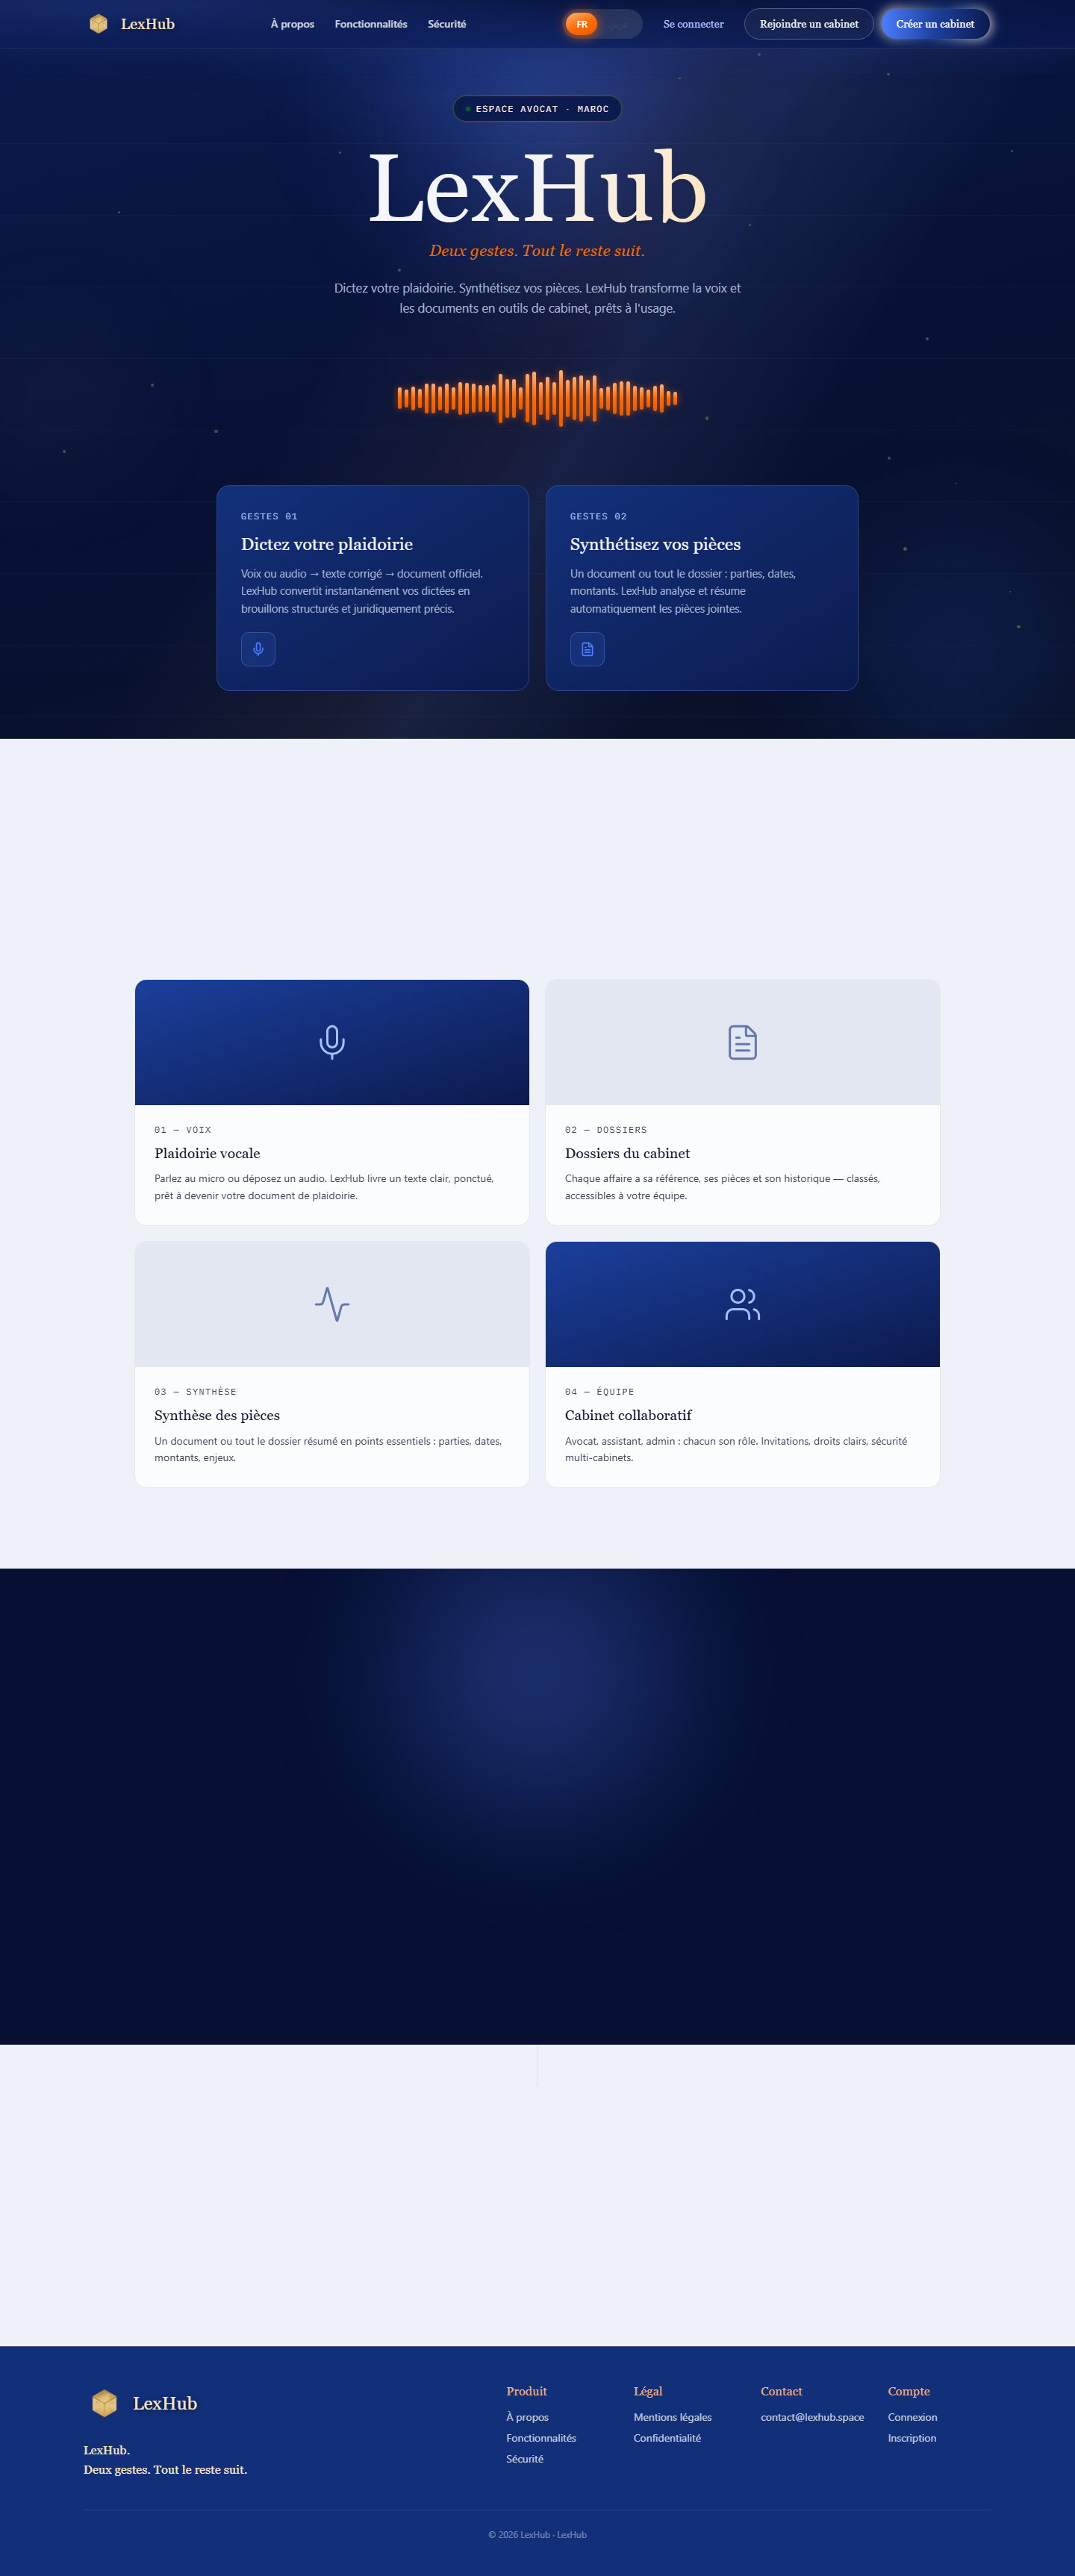
\includegraphics[width=0.98\textwidth]{screenshots/01-accueil.png}%
  }{\fbox{\rule{0pt}{3cm}\rule{5cm}{0pt}}}
  \par{\scriptsize\textbf{Accueil public}}
\end{column}
\begin{column}{0.48\textwidth}
  \centering
  \IfFileExists{screenshots/11-dossiers.png}{%
    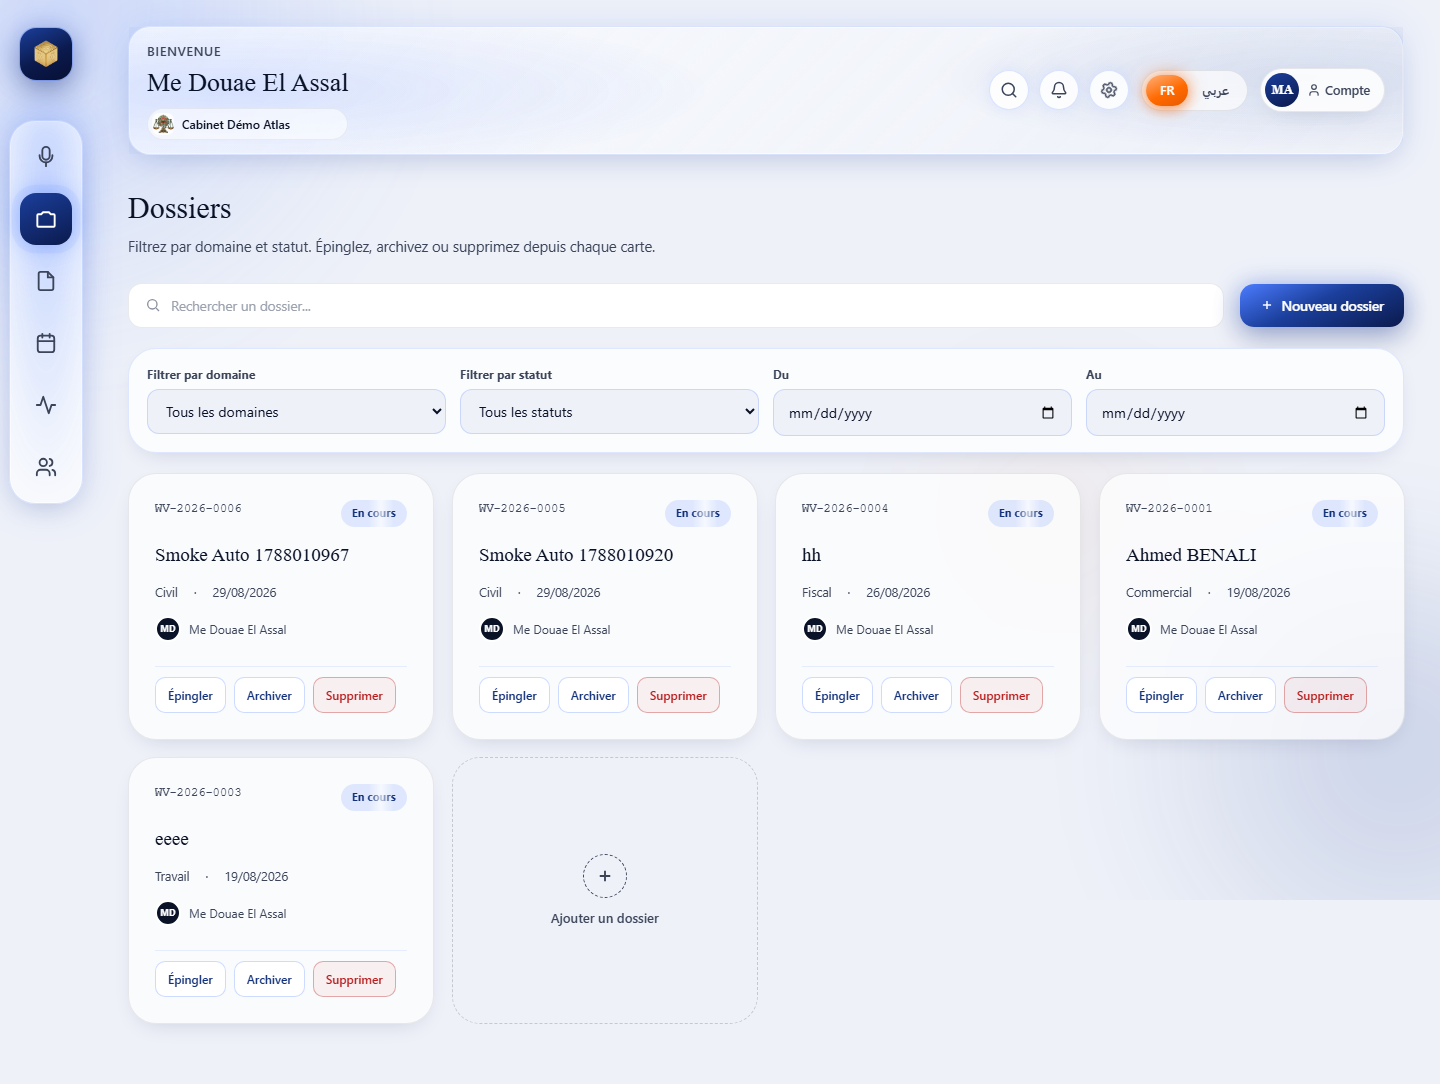
\includegraphics[width=0.98\textwidth]{screenshots/11-dossiers.png}%
  }{\fbox{\rule{0pt}{3cm}\rule{5cm}{0pt}}}
  \par{\scriptsize\textbf{Dossiers judiciaires}}
\end{column}
\end{columns}
\end{frame}

\begin{frame}{Démonstration --- Atelier}
\begin{columns}[T,onlytextwidth]
\begin{column}{0.48\textwidth}
  \centering
  \IfFileExists{screenshots/14b-plaidoirie-workspace.png}{%
    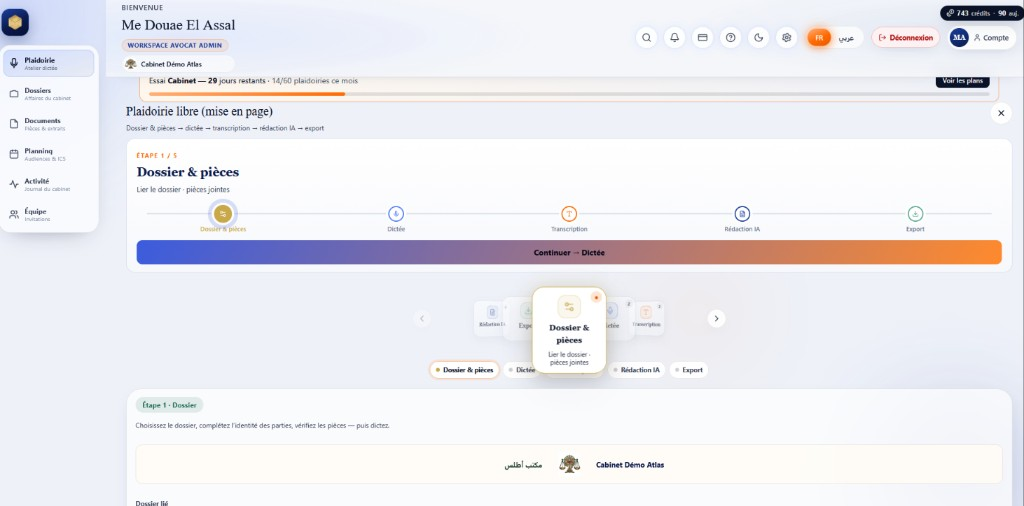
\includegraphics[width=0.98\textwidth]{screenshots/14b-plaidoirie-workspace.png}%
  }{\fbox{\rule{0pt}{3cm}\rule{5cm}{0pt}}}
  \par{\scriptsize\textbf{Workspace 5 étapes}}
\end{column}
\begin{column}{0.48\textwidth}
  \centering
  \IfFileExists{screenshots/14c-transcription-fusha.png}{%
    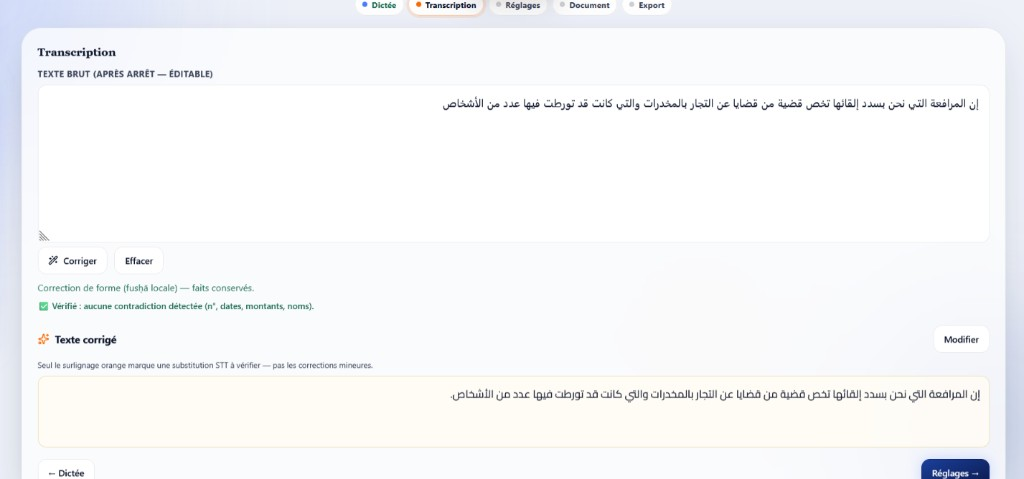
\includegraphics[width=0.98\textwidth]{screenshots/14c-transcription-fusha.png}%
  }{\fbox{\rule{0pt}{3cm}\rule{5cm}{0pt}}}
  \par{\scriptsize\textbf{Correction de forme}}
\end{column}
\end{columns}
\end{frame}

\begin{frame}{Démonstration --- Export \& Équipe}
\begin{columns}[T,onlytextwidth]
\begin{column}{0.48\textwidth}
  \centering
  \IfFileExists{screenshots/19-export-document.png}{%
    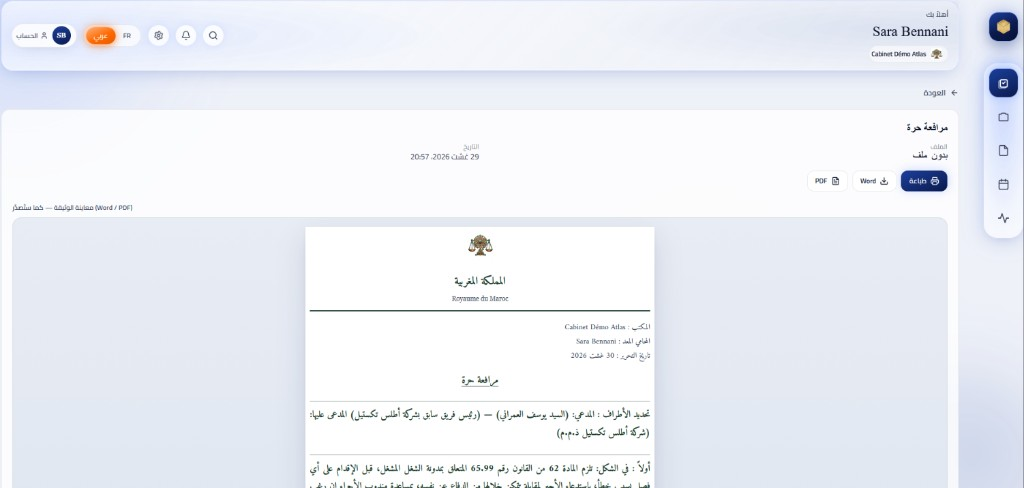
\includegraphics[width=0.98\textwidth]{screenshots/19-export-document.png}%
  }{\fbox{\rule{0pt}{3cm}\rule{5cm}{0pt}}}
  \par{\scriptsize\textbf{Export Word (.docx)}}
\end{column}
\begin{column}{0.48\textwidth}
  \centering
  \IfFileExists{screenshots/16-equipe.png}{%
    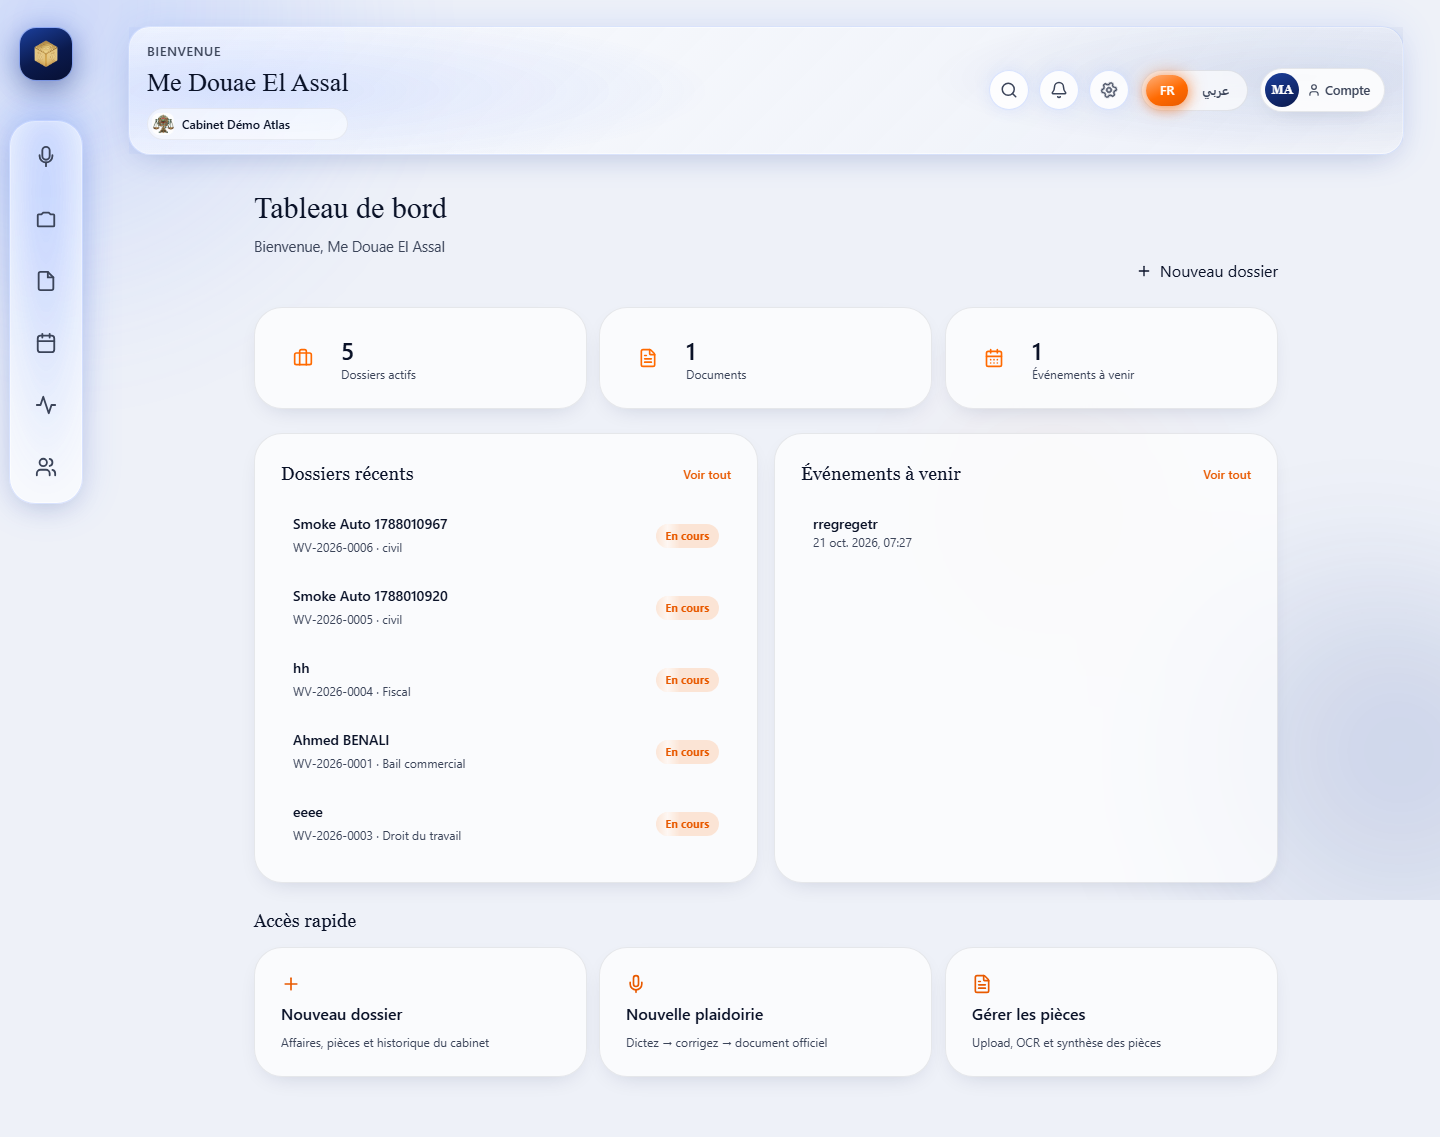
\includegraphics[width=0.98\textwidth]{screenshots/16-equipe.png}%
  }{\fbox{\rule{0pt}{3cm}\rule{5cm}{0pt}}}
  \par{\scriptsize\textbf{Équipe \& rôles}}
\end{column}
\end{columns}
\end{frame}

% =============================================================================
\section{Bilan \& Perspectives}

\begin{frame}{Bilan}
\framesubtitle{Objectifs PFA --- conformité}

\begin{table}
\small
\begin{tabular}{@{}p{5.6cm}p{5.8cm}c@{}}
\toprule
\textbf{Objectif} & \textbf{Livré} & \textbf{} \\
\midrule
Atelier 5 étapes & Dossier $\rightarrow$ Word & \badgegreen{OK} \\
SI multi-tenant + RBAC & Isolation + validation assistant & \badgegreen{OK} \\
Urbanisation MADI & Process / apps / données / infra & \badgegreen{OK} \\
Modèle économique & Essai, plans, packs, parrainage & \badgegreen{OK} \\
Production & \produrl & \badgegreen{OK} \\
\bottomrule
\end{tabular}
\end{table}
\end{frame}

\begin{frame}{Perspectives}
\framesubtitle{Évolution produit (hors périmètre PFA déjà livré)}

\begin{columns}[T,onlytextwidth]
\begin{column}{0.48\textwidth}
  \begin{block}{Court terme}
    \begin{itemize}
      \item Encaissement réel (CMI / PayZone).
      \item Qualité STT / relecture renforcée.
    \end{itemize}
  \end{block}
\end{column}
\begin{column}{0.48\textwidth}
  \begin{exampleblock}{Moyen terme}
    \begin{itemize}
      \item Continuité dossier $\rightarrow$ audience.
      \item Interopérabilités sans casser les maîtres de donnée.
    \end{itemize}
  \end{exampleblock}
\end{column}
\end{columns}

\medskip
\centering
\badgeblue{SI cabinet}\quad\badgegold{IA au service du métier}
\end{frame}

\begin{frame}[plain,noframenumbering]
  \begin{tikzpicture}[remember picture,overlay]
    \fill[UAEDarkBlue] (current page.south west)
      rectangle (current page.north east);
  \end{tikzpicture}
  \begin{center}
    \vspace{2.2cm}
    {\LARGE\bfseries\color{white} Merci pour votre attention}\\[0.5cm]
    {\large\bfseries\color{UAEAccentGold} Questions \& échanges}\\[0.8cm]
    {\normalsize\color{white!90}\textbf{EL ASSAL Douae} · Génie Informatique}\\[0.15cm]
    {\small\color{UAESkyBlue} ENSA Tétouan · WEBVOICE Tanger}\\[0.45cm]
    {\footnotesize\color{white!90}\textbf{Live :} \url{https://lexhub.space}}\\[0.15cm]
    {\scriptsize\color{white!70}\githubrepo}
  \end{center}
\end{frame}

\end{document}
